\documentclass{ximera}
\usepackage{epsfig}

\graphicspath{
  {./}
  {figures/}
}


\usepackage{morewrites}

%\newcounter{ccounter}
%\setcounter{ccounter}{1}
%\newcommand{\Chapter}[1]{\setcounter{chapter}{\arabic{ccounter}}\chapter{#1}\addtocounter{ccounter}{1}}

%\newcommand{\section}[1]{\section{#1}\setcounter{thm}{0}\setcounter{equation}{0}}

%\renewcommand{\theequation}{\arabic{chapter}.\arabic{section}.\arabic{equation}}
%\renewcommand{\thefigure}{\arabic{chapter}.\arabic{figure}}
%\renewcommand{\thetable}{\arabic{chapter}.\arabic{table}}

%\newcommand{\Sec}[2]{\section{#1}\markright{\arabic{ccounter}.\arabic{section}.#2}\setcounter{equation}{0}\setcounter{thm}{0}\setcounter{figure}{0}}

\newcommand{\Sec}[2]{\section{#1}}

\setcounter{secnumdepth}{2}
%\setcounter{secnumdepth}{1} 

%\newcounter{THM}
%\renewcommand{\theTHM}{\arabic{chapter}.\arabic{section}}

\newcommand{\trademark}{{R\!\!\!\!\!\bigcirc}}
%\newtheorem{exercise}{}

\newcommand{\dfield}{{\sf dfield9}}
\newcommand{\pplane}{{\sf pplane9}}

\newcommand{\EXER}{\section*{Exercises}}%\vspace*{0.2in}\hrule\small\setcounter{exercise}{0}}
\newcommand{\CEXER}{}%\vspace{0.08in}\begin{center}Computer Exercises\end{center}}
\newcommand{\TEXER}{} %\vspace{0.08in}\begin{center}Hand Exercises\end{center}}
\newcommand{\AEXER}{} %\vspace{0.08in}\begin{center}Hand Exercises\end{center}}

% BADBAD: \newcommand{\Bbb}{\bf}

\newcommand{\R}{\mbox{$\Bbb{R}$}}
\newcommand{\C}{\mbox{$\Bbb{C}$}}
\newcommand{\Z}{\mbox{$\Bbb{Z}$}}
\newcommand{\N}{\mbox{$\Bbb{N}$}}
\newcommand{\D}{\mbox{{\bf D}}}
\usepackage{amssymb}
%\newcommand{\qed}{\hfill\mbox{\raggedright$\square$} \vspace{1ex}}
%\newcommand{\proof}{\noindent {\bf Proof:} \hspace{0.1in}}

\newcommand{\setmin}{\;\mbox{--}\;}
\newcommand{\Matlab}{{M\small{AT\-LAB}} }
\newcommand{\Matlabp}{{M\small{AT\-LAB}}}
\newcommand{\computer}{\Matlab Instructions}
\newcommand{\half}{\mbox{$\frac{1}{2}$}}
\newcommand{\compose}{\raisebox{.15ex}{\mbox{{\scriptsize$\circ$}}}}
\newcommand{\AND}{\quad\mbox{and}\quad}
\newcommand{\vect}[2]{\left(\begin{array}{c} #1_1 \\ \vdots \\
 #1_{#2}\end{array}\right)}
\newcommand{\mattwo}[4]{\left(\begin{array}{rr} #1 & #2\\ #3
&#4\end{array}\right)}
\newcommand{\mattwoc}[4]{\left(\begin{array}{cc} #1 & #2\\ #3
&#4\end{array}\right)}
\newcommand{\vectwo}[2]{\left(\begin{array}{r} #1 \\ #2\end{array}\right)}
\newcommand{\vectwoc}[2]{\left(\begin{array}{c} #1 \\ #2\end{array}\right)}



\newcommand{\inv}{^{-1}}
\newcommand{\CC}{{\cal C}}
\newcommand{\CCone}{\CC^1}
\newcommand{\Span}{{\rm span}}
\newcommand{\rank}{{\rm rank}}
\newcommand{\trace}{{\rm tr}}
\newcommand{\RE}{{\rm Re}}
\newcommand{\IM}{{\rm Im}}
\newcommand{\nulls}{{\rm null\;space}}

\newcommand{\dps}{\displaystyle}
\newcommand{\arraystart}{\renewcommand{\arraystretch}{1.8}}
\newcommand{\arrayfinish}{\renewcommand{\arraystretch}{1.2}}
\newcommand{\Start}[1]{\vspace{0.08in}\noindent {\bf Section~\ref{#1}}}
\newcommand{\exer}[1]{\noindent {\bf \ref{#1}}}
\newcommand{\ans}{}
\newcommand{\matthree}[9]{\left(\begin{array}{rrr} #1 & #2 & #3 \\ #4 & #5 & #6
\\ #7 & #8 & #9\end{array}\right)}
\newcommand{\cvectwo}[2]{\left(\begin{array}{c} #1 \\ #2\end{array}\right)}
\newcommand{\cmatthree}[9]{\left(\begin{array}{ccc} #1 & #2 & #3 \\ #4 & #5 &
#6 \\ #7 & #8 & #9\end{array}\right)}
\newcommand{\vecthree}[3]{\left(\begin{array}{r} #1 \\ #2 \\
#3\end{array}\right)}
\newcommand{\cvecthree}[3]{\left(\begin{array}{c} #1 \\ #2 \\
#3\end{array}\right)}
\newcommand{\cmattwo}[4]{\left(\begin{array}{cc} #1 & #2\\ #3
&#4\end{array}\right)}

\newcommand{\Matrix}[1]{\ensuremath{\left(\begin{array}{rrrrrrrrrrrrrrrrrr} #1 \end{array}\right)}}

\newcommand{\Matrixc}[1]{\ensuremath{\left(\begin{array}{cccccccccccc} #1 \end{array}\right)}}



\renewcommand{\labelenumi}{\theenumi)}
\newenvironment{enumeratea}%
{\begingroup
 \renewcommand{\theenumi}{\alph{enumi}}
 \renewcommand{\labelenumi}{(\theenumi)}
 \begin{enumerate}}
 {\end{enumerate}\endgroup}



\newcounter{help}
\renewcommand{\thehelp}{\thesection.\arabic{equation}}

%\newenvironment{equation*}%
%{\renewcommand\endequation{\eqno (\theequation)* $$}%
%   \begin{equation}}%
%   {\end{equation}\renewcommand\endequation{\eqno \@eqnnum
%$$\global\@ignoretrue}}

%\input{psfig.tex}

\author{Martin Golubitsky and Michael Dellnitz}

%\newenvironment{matlabEquation}%
%{\renewcommand\endequation{\eqno (\theequation*) $$}%
%   \begin{equation}}%
%   {\end{equation}\renewcommand\endequation{\eqno \@eqnnum
% $$\global\@ignoretrue}}

\newcommand{\soln}{\textbf{Solution:} }
\newcommand{\exercap}[1]{\centerline{Figure~\ref{#1}}}
\newcommand{\exercaptwo}[1]{\centerline{Figure~\ref{#1}a\hspace{2.1in}
Figure~\ref{#1}b}}
\newcommand{\exercapthree}[1]{\centerline{Figure~\ref{#1}a\hspace{1.2in}
Figure~\ref{#1}b\hspace{1.2in}Figure~\ref{#1}c}}
\newcommand{\para}{\hspace{0.4in}}

\renewenvironment{solution}{\suppress}{\endsuppress}

\ifxake
\newenvironment{matlabEquation}{\begin{equation}}{\end{equation}}
\else
\newenvironment{matlabEquation}%
{\let\oldtheequation\theequation\renewcommand{\theequation}{\oldtheequation*}\begin{equation}}%
  {\end{equation}\let\theequation\oldtheequation}
\fi

\makeatother

\begin{document}

\noindent In Exercises~\ref{E:PPa} -- \ref{E:PPe}, consider the four pictures
in Figure~\ref{F:PP}.  Each picture is a phase portrait of a system of
differential equations $\dot{X}=CX$ where $C$ is a $2\times 2$ matrix.  Answer
the given question for each of these phase portraits.
\begin{exercise}  \label{E:PPa}
What is the name of the type of equilibrium at the origin?

\begin{solution}
\ans System $A$ has a spiral sink at the origin, $B$ has a
saddle, $C$ has a saddle node, and $D$ has an improper nodal source.

\soln Answers can be determined visually using the graphs and examples
from Sections~\ref{S:PlanarSystems} and \ref{S:6.9} of the text.

\end{solution}
\end{exercise}
\begin{exercise}  \label{E:PPb}
Is the origin asymptotically stable?

\begin{solution}
\ans The origin is asymptotically stable for $A$ and unstable
for $B$, $C$ and $D$.

\soln The origin is asymptotically stable if all solutions tend towards
the origin as $t \rightarrow \infty$.

\end{solution}
\end{exercise}
\begin{exercise}  \label{E:PPc}
Is ${\rm trace}(C)$ positive, negative, or zero?

\begin{solution}
\ans The traces of $A$, $B$ and $C$ are negative, and the
trace of $D$ is positive.

\soln The trace of a matrix is the sum of the eigenvalues, so the trace
is positive for sources, which have two positive eigenvalues and
negative for sinks, which have two negative eigenvalues.  The trajectories
of $C$ approach the eigenvector of $0$ as $t$ increases, rather
than tending away from it, so the nonzero eigenvector is negative and,
therefore, the trace is also negative.

\end{solution}
\end{exercise}
\begin{exercise}  \label{E:PPd}
Is $\det(C)$ positive, negative, or zero?

\begin{solution}
\ans The determinants of $A$ and $D$ are positive, the
determinant of $B$ is negative, and the determinant of $C$ is zero.

\soln The determinant of a matrix is the product of the eigenvectors.  The
eigenvectors of $A$ are complex conjugates, so their product
is positive.  A saddle has one negative and one positive eigenvector, so
the determinant of $B$ is negative.  A saddle node has one zero
eigenvector, so the product of the eigenvectors of $C$ is zero.  An
improper nodal source has equal positive eigenvectors, so the determinant
of $D$ is positive.

\end{solution}
\end{exercise}
\begin{exercise}  \label{E:PPe}
Is ${\rm discriminant}(C)$ positive, negative, or zero?

\begin{solution}
\ans The discriminant of $A$ is negative, the discriminants of
$B$ and $C$ are positive, and the discriminant of $D$ is zero.

\soln The discriminant of a matrix is negative when the eigenvalues are
a complex conjugate pair, positive when the eigenvalues are real, and
zero when the eigenvalues are equal.

\end{solution}
\end{exercise}

\begin{figure*}[htb]
\centerline{(A) \hspace{2.7in} (B)}
           \centerline{%
           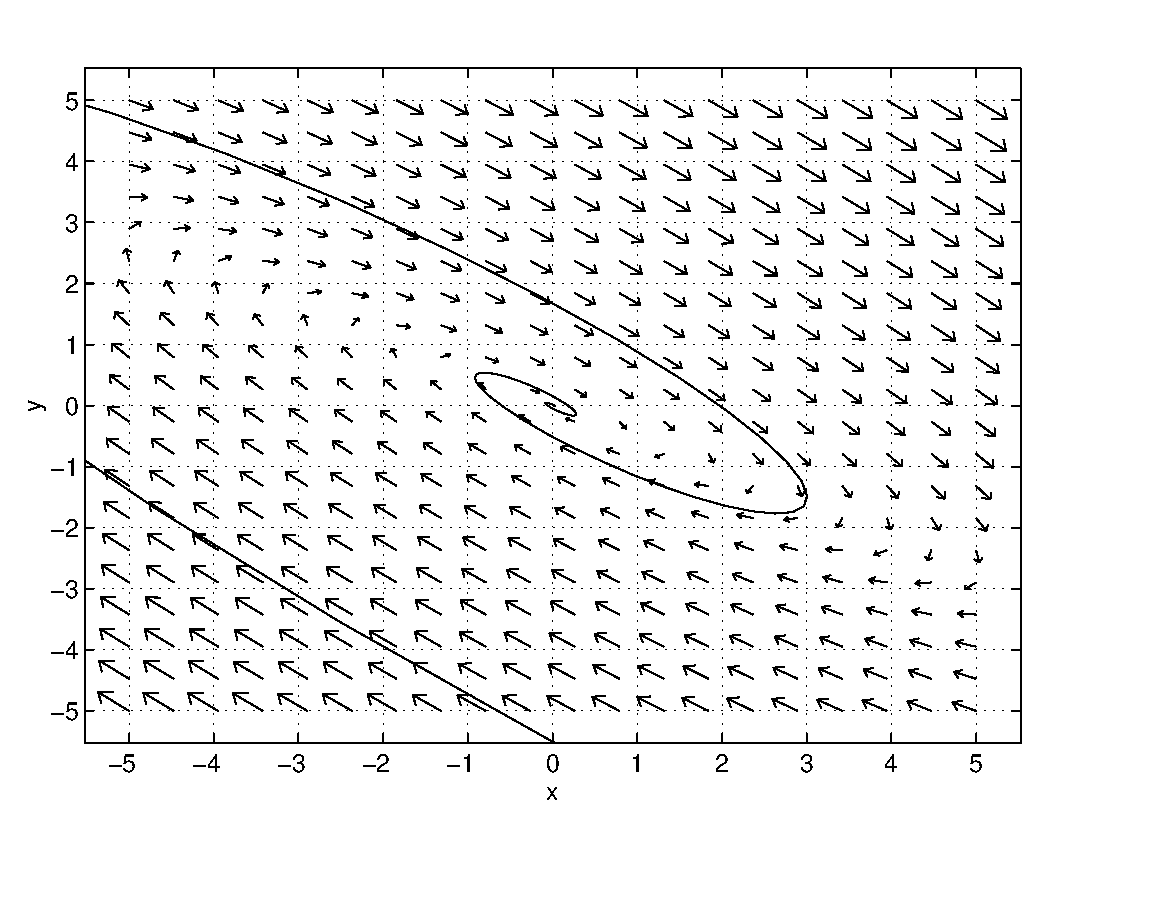
\psfig{file=../figures/e2B.eps,width=3.0in}
           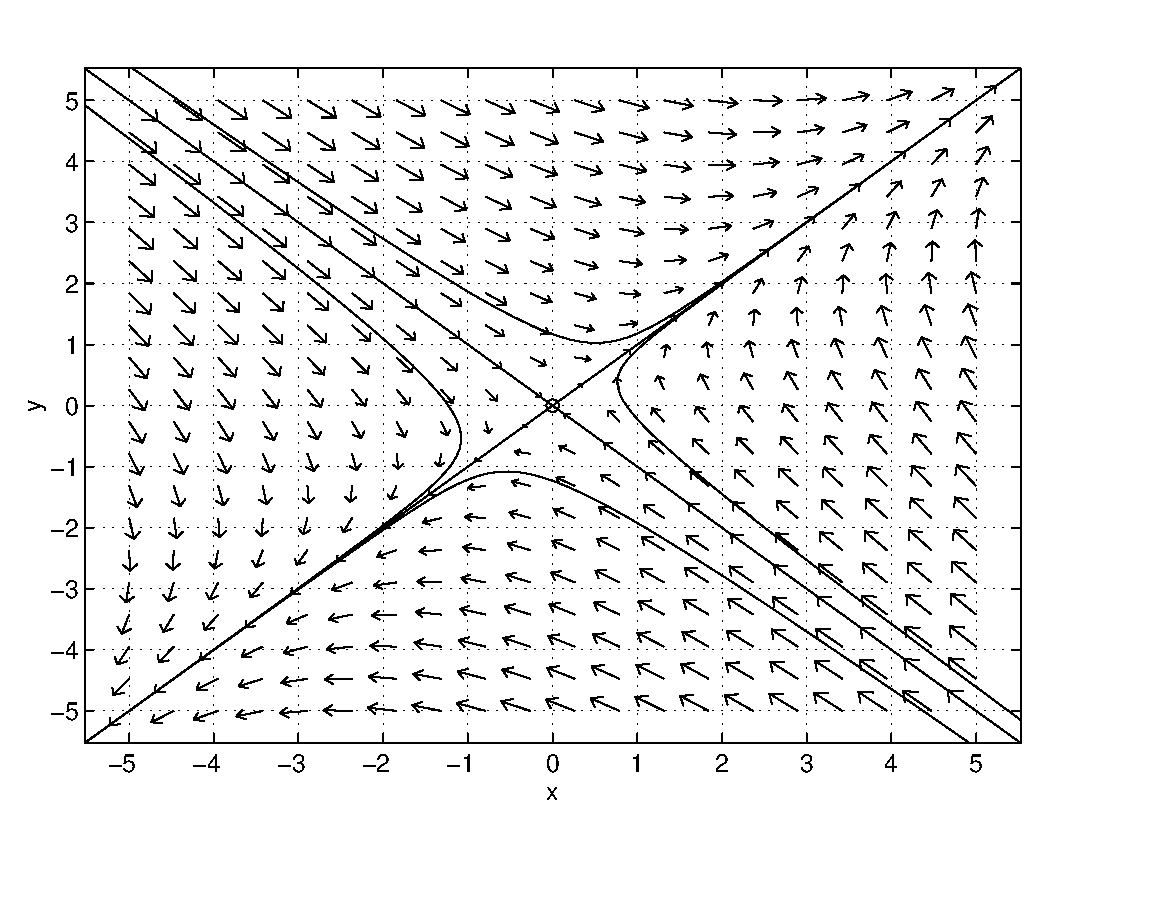
\psfig{file=../figures/e2C.eps,width=3.0in}}
\centerline{(C) \hspace{2.7in} (D)}
           \centerline{%
           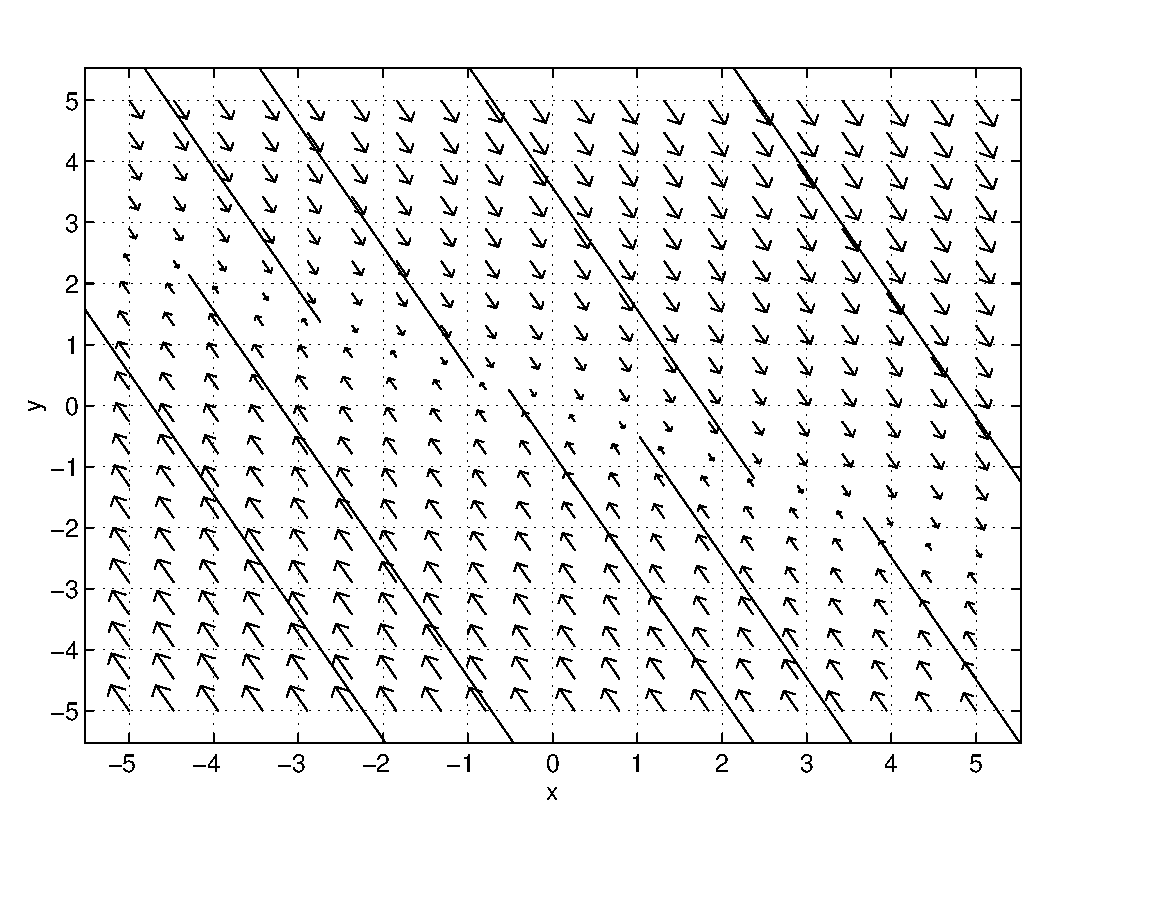
\psfig{file=../figures/e2A.eps,width=3.0in}
           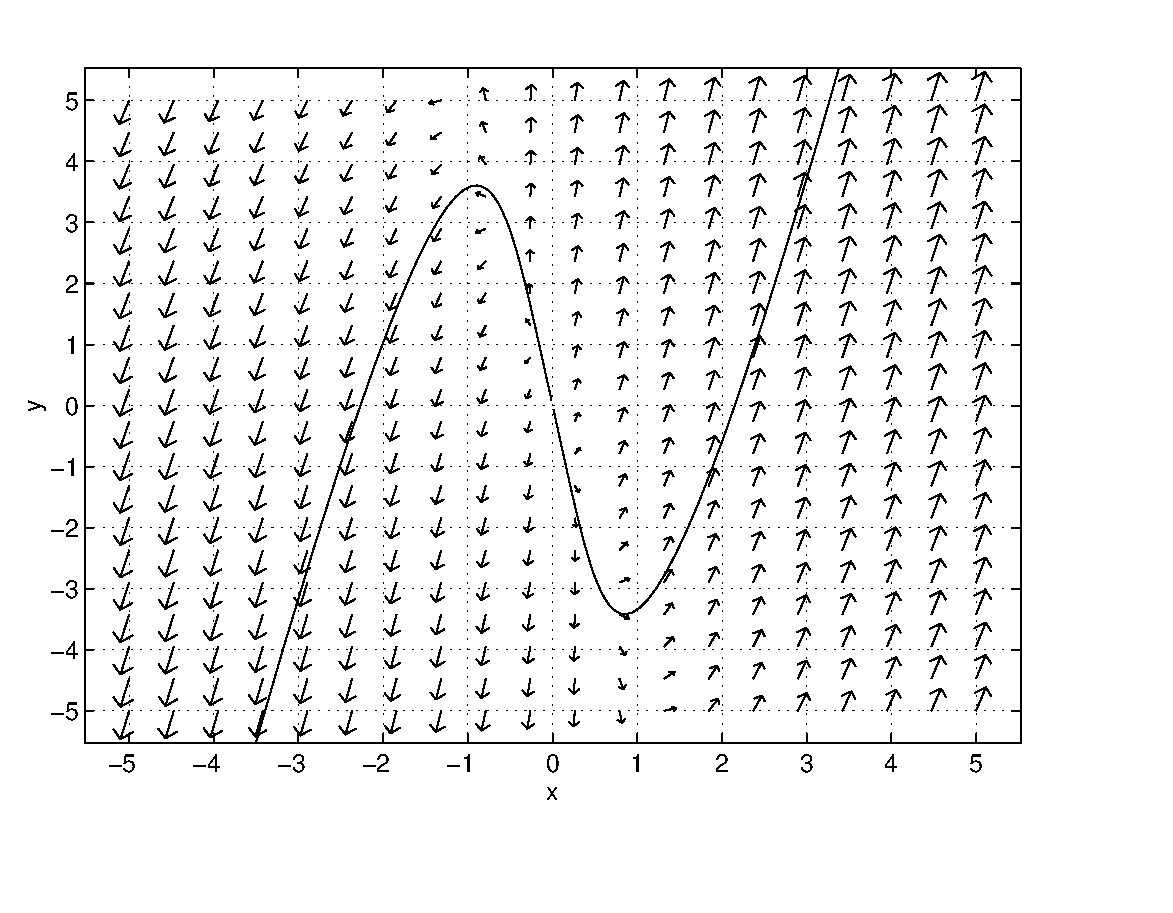
\psfig{file=../figures/e2D.eps,width=3.0in}}
\caption{Phase portraits for planar linear systems in
Exercises~\protect\ref{E:PPa} -- \protect\ref{E:PPe}}
\label{F:PP}
\end{figure*}

\noindent In Exercises~\ref{E:PQa} -- \ref{E:PQg}, consider the system of
differential equations $\dot{X}=CX$ where $C$ is the given matrix.  For each
system determine whether the origin is hyperbolic or not and the type of
equilibrium at the origin (spiral sink, center, etc.).
\end{document}
